% KnowledgeMind — ECAI-style 3-page project report
% Compile: pdflatex -> bibtex -> pdflatex -> pdflatex
\documentclass[10pt,twocolumn]{article}

% ── Geometry & fonts ──────────────────────────────────────────────────────────
\usepackage[a4paper,
            top=2.4cm, bottom=2.4cm,
            left=1.7cm, right=1.7cm,
            columnsep=0.6cm]{geometry}
\usepackage{times}
\usepackage[T1]{fontenc}
\usepackage[utf8]{inputenc}
\usepackage{microtype}

% ── Headings & layout ─────────────────────────────────────────────────────────
\usepackage{titlesec}
\titleformat{\section}{\normalsize\bfseries\scshape}{\thesection.}{0.5em}{}
\titleformat{\subsection}{\small\bfseries}{\thesubsection}{0.5em}{}
\titlespacing*{\section}{0pt}{6pt}{3pt}
\titlespacing*{\subsection}{0pt}{4pt}{2pt}

% ── Graphics, diagrams, tables ────────────────────────────────────────────────
\usepackage{graphicx}
\usepackage{tikz}
\usetikzlibrary{shapes.geometric, arrows.meta, positioning, fit,
                backgrounds, decorations.pathreplacing, calc}
\usepackage{booktabs}
\usepackage{tabularx}
\usepackage{xcolor}

% ── References & hyperlinks ───────────────────────────────────────────────────
\usepackage{cite}
\usepackage[hidelinks]{hyperref}

% ── Utility ───────────────────────────────────────────────────────────────────
\usepackage{parskip}
\setlength{\parskip}{2pt}
\setlength{\parindent}{1em}
\usepackage{enumitem}
\setlist{nosep, leftmargin=1.2em}

% ── Colour palette ────────────────────────────────────────────────────────────
\definecolor{localcol}{HTML}{2E86AB}   % steel blue  – local/private
\definecolor{cloudcol}{HTML}{E87722}   % amber       – cloud
\definecolor{kgcol}{HTML}{4C956C}      % green       – knowledge graph
\definecolor{agentcol}{HTML}{6A4C93}   % purple      – agent
\definecolor{conncol}{HTML}{C77DFF}    % lavender    – connectors
\definecolor{monoccol}{HTML}{F4A261}   % warm orange – monitor
\definecolor{headercol}{HTML}{1A1A2E}  % near-black  – headers

% ─────────────────────────────────────────────────────────────────────────────
%  TITLE BLOCK
% ─────────────────────────────────────────────────────────────────────────────
\title{\textbf{KnowledgeMind: A Privacy-Aware Hybrid AI Agent\\
for Organisational Commitment and Knowledge Management}}

\author{%
  Aarif Zafar\quad
  Swarup E\quad
  Rakshit Ramesh\quad
  Novoneel Chakraborty\\
  Sourav Thakur\quad
  Sathya Sekar\quad
  Sarthak Sharma\\[2pt]
  \small Department of Computational and Data Sciences\\
  \small Indian Institute of Science, Bengaluru 560012, India
}
\date{}

\begin{document}
\maketitle
\thispagestyle{empty}

% ─────────────────────────────────────────────────────────────────────────────
%  ABSTRACT
% ─────────────────────────────────────────────────────────────────────────────
\begin{abstract}
\noindent
Professionals operating across multiple communication channels accumulate
implicit commitments—meeting agreements, task deadlines, informal promises—that
existing productivity tools fail to track holistically.
We present \textbf{KnowledgeMind}, a privacy-aware personal AI agent that
ingests Slack, calendar, and e-mail streams, extracts hard and soft commitments
via spaCy NER and few-shot prompted LLMs, and fuses them into a
SQLite\,+\,NetworkX personal knowledge graph.
A proactive LangGraph FSM monitors the graph for temporal conflicts and nudges
the user before they arise.
A hybrid privacy router enforces an invariant: any task touching personal data
is executed exclusively on a local Qwen2.5-3B model; only non-sensitive tasks
are delegated to a free-tier cloud model.
A three-level ReAct agent (L1–L3) and a Project Advisor sub-system extend the
platform into full organisational project management.
The system runs CPU-only on commodity hardware and degrades gracefully to mock
data in the absence of API keys.
\end{abstract}

% ─────────────────────────────────────────────────────────────────────────────
%  1  INTRODUCTION
% ─────────────────────────────────────────────────────────────────────────────
\section{Introduction}

Modern knowledge workers routinely context-switch across e-mail, instant
messaging, and calendar applications.
This fragmentation creates a structural blind spot: commitments that exist
across channels—``I'll have the report ready by Friday'' in Slack,
a 3\,PM meeting in Google Calendar, a task in a project tracker—are never
co-located, so conflicts remain invisible until they escalate into missed
deadlines or double-booked time.

Existing solutions address only one slice of this problem.
Calendar applications are authoritative for hard, confirmed events but ignore
the conversational layer.
Task managers such as Todoist or Notion require \emph{manual} entry and are
therefore only as complete as the user's discipline.
Large-language-model (LLM) assistants such as ChatGPT or Copilot can
summarise or draft content but lack persistent memory, have no live connection
to personal data sources, and route \emph{all} user data to external servers,
creating unacceptable privacy exposure.

\medskip\noindent\textbf{Problem statement.}
Given a heterogeneous stream of communication artefacts (chat messages,
calendar events, e-mails), the system must: (i)~extract implicit and explicit
commitments from natural language; (ii)~fuse them into a temporally consistent
personal knowledge graph; (iii)~detect and proactively surface conflicts;
and (iv)~do so without transmitting personal data beyond the user's device.

\medskip\noindent\textbf{Contributions.}
\begin{enumerate}
  \item A privacy-invariant hybrid router that guarantees personal data never
        leaves the local model, with per-tool minimum privacy floors.
  \item A dual-tier commitment extraction pipeline combining spaCy NER and
        few-shot LLM prompting with confidence-graded output
        (HARD / SOFT / TENTATIVE).
  \item A proactive LangGraph FSM that monitors the KG autonomously, detects
        temporal overlaps, and emits dismissable nudges with quiet-hour
        suppression.
  \item A three-level ReAct orchestrator and an integrated Project Advisor that
        together span L1 single-shot to L3 multi-step replanning.
\end{enumerate}

% ─────────────────────────────────────────────────────────────────────────────
%  2  RELATED WORK AND MARKET LANDSCAPE
% ─────────────────────────────────────────────────────────────────────────────
\section{Related Work and Market Landscape}

\subsection{Existing Productivity and AI Tools}

Table~\ref{tab:comparison} maps the most prominent competing tools against the
capabilities that KnowledgeMind targets.

\begin{table}[h]
\centering
\caption{Feature comparison across competing tools.}
\label{tab:comparison}
\renewcommand{\arraystretch}{1.15}
{\tiny
\setlength{\tabcolsep}{2.5pt}
\begin{tabular}{@{}l ccccc@{}}
\toprule
\textbf{Feature} &
\rotatebox{65}{\textbf{Notion AI}} &
\rotatebox{65}{\textbf{Copilot}} &
\rotatebox{65}{\textbf{ChatGPT}} &
\rotatebox{65}{\textbf{Todoist}} &
\rotatebox{65}{\textbf{KM (Ours)}} \\
\midrule
Cross-channel ingestion    & $\times$ & \checkmark & $\times$ & $\times$ & \checkmark \\
Soft-commit.\ extraction   & $\times$ & $\times$   & $\times$ & $\times$ & \checkmark \\
Conflict detection         & $\times$ & partial    & $\times$ & $\times$ & \checkmark \\
Proactive alerting         & $\times$ & $\times$   & $\times$ & $\times$ & \checkmark \\
On-device privacy          & $\times$ & $\times$   & $\times$ & \checkmark & \checkmark \\
Persistent KG memory       & partial  & $\times$   & plugin   & $\times$ & \checkmark \\
Project plan alignment     & partial  & $\times$   & $\times$ & partial  & \checkmark \\
CPU-only / free            & $\times$ & $\times$   & $\times$ & partial  & \checkmark \\
\bottomrule
\end{tabular}
}
\end{table}

\noindent\textbf{Notion AI / Confluence.}
Document-centric wikis with AI-assisted drafting.
They require manual data entry and do not ingest live communication
channels~\cite{notion2024}.

\noindent\textbf{Microsoft Copilot for Microsoft 365.}
Deep integration with the M365 ecosystem provides meeting summaries and
e-mail drafting, but all inference runs on Microsoft's cloud servers, data
is not retained in a user-controlled graph, and the service is subscription
gated~\cite{ms2024copilot}.

\noindent\textbf{ChatGPT / Gemini.}
Powerful conversational AI with optional plugin ecosystems.
No persistent cross-session memory by default, no proactive alerting, and full
data egress to external servers~\cite{openai2024gpt4}.

\noindent\textbf{Todoist / Linear / Jira.}
Task and project trackers that enforce structured, manual workflows.
They capture only data the user explicitly enters and provide no NLP-based
extraction from conversational channels.

\subsection{Why a Unified Solution is Needed}

Each existing tool covers at most one or two of the five axes:
\emph{ingestion, extraction, memory, privacy, proactivity}.
A practitioner who wants all five must manually stitch together multiple
subscriptions and accept that personal data flows to multiple cloud providers.
KnowledgeMind is designed as a single, locally running agent that closes all
five gaps simultaneously, while remaining extensible via a Model Context
Protocol (MCP) server for third-party tool integration.

% ─────────────────────────────────────────────────────────────────────────────
%  3  PROPOSED METHODOLOGY
% ─────────────────────────────────────────────────────────────────────────────
\section{Proposed Methodology}

\subsection{System Architecture}

Figure~\ref{fig:arch} illustrates the end-to-end architecture.
The system decomposes into five interacting layers:
\emph{Connectors}, \emph{Extraction}, \emph{Knowledge Graph},
\emph{Routing \& Agent}, and \emph{Interface}.

\begin{figure}[h]
\centering
\resizebox{\columnwidth}{!}{%
\begin{tikzpicture}[
  font=\scriptsize,
  >=Stealth,
  every node/.style={align=center},
  box/.style={draw, rounded corners=3pt, minimum width=2.1cm,
              minimum height=0.55cm, inner sep=3pt, font=\scriptsize\bfseries},
  smallbox/.style={draw, rounded corners=2pt, minimum width=1.6cm,
                   minimum height=0.45cm, inner sep=2pt, font=\tiny},
  arr/.style={->, thick},
  grp/.style={draw, dashed, rounded corners=5pt, inner sep=5pt}
]

%% ── Row 0 : Channels ──────────────────────────────────────────────────────
\node[box, fill=conncol!20, draw=conncol] (slack)   at (0,   0)    {Slack};
\node[box, fill=conncol!20, draw=conncol] (cal)     at (2.3, 0)    {Calendar};
\node[box, fill=conncol!20, draw=conncol] (gmail)   at (4.6, 0)    {Gmail};
\node[box, fill=conncol!20, draw=conncol] (hermes)  at (6.9, 0)    {Hermes\\Signals};

\node[font=\tiny, above=0pt of slack, xshift=1.45cm]
      {\textit{Communication \& Signal Connectors}};

%% ── Row 1 : Monitor FSM ───────────────────────────────────────────────────
\node[box, fill=monoccol!25, draw=monoccol,
      minimum width=5.0cm] (monitor) at (2.3, -1.3)
      {Background Monitor FSM\\{\tiny POLL$\!\to\!$EXTRACT$\!\to\!$UPDATE$\!\to\!$CHECK$\!\to\!$ALERT}};

\foreach \s in {slack, cal, gmail}
  \draw[arr, color=conncol] (\s.south) -- +(0,-0.3) -| (monitor.north);
\draw[arr, color=conncol, dashed] (hermes.south) -- +(0,-0.55)
      node[right, font=\tiny, yshift=0.2cm]{agent\\tools} +(0,0);

%% ── Row 1b : Extraction ───────────────────────────────────────────────────
\node[box, fill=gray!15, draw=gray!60,
      minimum width=4.6cm] (extract) at (2.3, -2.35)
      {Extraction Pipeline\\{\tiny spaCy NER + Few-Shot LLM $\to$ HARD / SOFT / TENTATIVE}};

\draw[arr] (monitor.south) -- (extract.north);

%% ── Row 2 : Knowledge Graph ───────────────────────────────────────────────
\node[box, fill=kgcol!20, draw=kgcol,
      minimum width=6.8cm] (kg) at (3.45, -3.4)
      {Personal Knowledge Graph (SQLite + NetworkX)\\
       {\tiny Person $\xrightarrow{\text{has}}$ Commitment $\xrightarrow{\text{at}}$ TimeSlot; conflict edges auto-inserted}};

\draw[arr, color=kgcol] (extract.south) -- (kg.north);

%% ── Row 3 : Router ────────────────────────────────────────────────────────
\node[box, fill=gray!10, draw=gray!70,
      minimum width=3.8cm] (router) at (1.9, -4.55)
      {Privacy Router\\{\tiny privacy score + complexity score}};

\draw[arr] (kg.south) -| (router.north);

%% LOCAL / CLOUD branches
\node[smallbox, fill=localcol!25, draw=localcol] (local) at (0.0, -5.75)
      {LOCAL\\{\tiny Qwen2.5-3B (Ollama)}};
\node[smallbox, fill=cloudcol!25, draw=cloudcol] (cloud) at (3.6, -5.75)
      {CLOUD\\{\tiny Llama-3.3-70B (Groq)}};

\draw[arr, color=localcol]  (router.south) -- +(-0.9,-0.4) -- (local.north);
\draw[arr, color=cloudcol]  (router.south) -- +(+1.7,-0.4) -- (cloud.north);

\node[font=\tiny, color=localcol, below=1pt of local, xshift=-4pt]
      {privacy $\geq$ 0.65};
\node[font=\tiny, color=cloudcol, below=1pt of cloud, xshift=4pt]
      {low priv + high complexity};

%% ── Row 4 : Agent ─────────────────────────────────────────────────────────
\node[box, fill=agentcol!20, draw=agentcol,
      minimum width=4.6cm] (agent) at (1.9, -7.05)
      {HybridMind ReAct Agent (L1 / L2 / L3)\\
       {\tiny Reason $\to$ Act $\to$ Observe $\to$ Replan; LangGraph orchestration}};

\draw[arr, color=localcol] (local.south) -- +(0,-0.35) -| (agent.north);
\draw[arr, color=cloudcol] (cloud.south) -- +(0,-0.35) -| (agent.north);

%% ── Row 5 : Tools + Proj Advisor ──────────────────────────────────────────
\node[smallbox, fill=agentcol!10, draw=agentcol,
      minimum width=2.7cm] (tools) at (0.5, -8.15)
      {Tool Registry\\{\tiny KG · RAG · Web · Calendar}};
\node[smallbox, fill=kgcol!15, draw=kgcol,
      minimum width=2.6cm] (pm) at (3.8, -8.15)
      {Project Advisor\\{\tiny SOW $\to$ KG $\to$ rules $\to$ chat}};

\draw[arr] (agent.south) -- +(-0.9,-0.35) -- (tools.north);
\draw[arr] (agent.south) -- +(+1.7,-0.35) -- (pm.north);

%% ── Row 6 : Interface ─────────────────────────────────────────────────────
\node[box, fill=gray!15, draw=gray!60,
      minimum width=6.2cm] (ui) at (2.2, -9.2)
      {React SPA + FastAPI (access-key auth, CORS, MCP server)\\
       {\tiny Briefing · Nudges · Conflict View · Connectors · Audit log}};

\draw[arr] (tools.south) |- (ui.west);
\draw[arr] (pm.south) |- (ui.east);

%% ── Proactive nudge feedback arc ──────────────────────────────────────────
\draw[arr, color=monoccol, dashed, bend left=40]
      (kg.east) to node[right, font=\tiny]{nudge\\outbox} (ui.east);

%% ── Group labels ──────────────────────────────────────────────────────────
\begin{scope}[on background layer]
  \node[grp, draw=conncol!50,  fill=conncol!5,
        fit=(slack)(cal)(gmail)(hermes)(monitor)(extract),
        label={[font=\tiny\color{conncol}]north west:Ingestion}] {};
  \node[grp, draw=agentcol!50, fill=agentcol!5,
        fit=(router)(local)(cloud)(agent)(tools)(pm),
        label={[font=\tiny\color{agentcol}]north west:Reasoning}] {};
\end{scope}

\end{tikzpicture}}%
\caption{KnowledgeMind system architecture.
  Blue boxes: local-only; amber: cloud-eligible; green: knowledge graph;
  purple: agent and reasoning; dashed arrows: asynchronous paths.}
\label{fig:arch}
\end{figure}

\subsection{Commitment Extraction}

Messages from each connector are passed through a two-stage pipeline.
First, spaCy's \texttt{en\_core\_web\_sm} model identifies named entities
(persons, dates, times, organisations).
Second, a few-shot prompted local LLM classifies each candidate span into one
of three commitment types: HARD (confirmed calendar events), SOFT
(conversational agreements, confidence $\geq 0.6$), or TENTATIVE (confidence
$< 0.6$).
The temporal expression resolver (\texttt{extraction/timeparse.py}) converts
relative expressions such as ``\emph{by end of day}'' into absolute ISO
timestamps for graph insertion.

\subsection{Privacy Router}

The router assigns two scores to each incoming task: a \emph{privacy score}
$p \in [0,1]$ computed from keyword and tool-type matching, and a
\emph{complexity score} $c \in [0,1]$ derived from structural heuristics
(multi-step keywords, clause count).
The decision rule is:

\begin{center}
\small
\begin{tabular}{@{}ll@{}}
  \textsc{local} & if $p \geq 0.65$ \;(privacy always wins)\\
  \textsc{cloud} & if $c \geq 0.6$ and $p < 0.65$\\
  \textsc{local} & otherwise (conservative fallback)
\end{tabular}
\end{center}

\medskip\noindent
A fixed set \texttt{ALWAYS\_LOCAL\_TOOLS} (KG queries, calendar, Gmail,
health/fitness signals) is never routed to the cloud regardless of scores.
Per-tool minimum privacy floors (e.g.\ KG $\geq 0.90$) make the invariant
immune to adversarial task phrasing.

\subsection{Three-Level ReAct Agent}

\textbf{L1} handles single-question tasks with one optional tool call and
direct synthesis.
\textbf{L2} (default) uses a cloud plan–local dispatch–cloud critique loop:
the cloud model generates a plan, each step is executed locally by
\texttt{dispatch\_tool}, and the cloud model critiques the result.
\textbf{L3} is a full LangGraph ReAct loop with automatic replanning on tool
failure: if a booked time slot is already occupied (conflict detected by the
KG), the agent finds the next free slot and retries.

\subsection{Project Advisor}

The Project Advisor is a self-contained ASGI sub-application mounted at
\texttt{/projmgmt}.
It accepts a Statement of Work document, builds a project-specific knowledge
graph with rules (scope, budget, schedule), and exposes a chat interface that
rates user queries against the project plan, flagging scope deviations with
confidence scores.
It shares the same privacy router and cloud LLM key as the main agent,
making organisational project governance a first-class citizen of the platform.

% ─────────────────────────────────────────────────────────────────────────────
%  4  CONCLUSION AND FUTURE PROSPECTS
% ─────────────────────────────────────────────────────────────────────────────
\section{Conclusion and Future Prospects}

\noindent\textbf{Summary.}
KnowledgeMind addresses a practical gap at the intersection of personal
information management and privacy-preserving AI.
By combining a live personal knowledge graph, a proactive conflict-aware
monitor, a provably private routing layer, and a multi-level ReAct agent, the
system provides a unified organisational intelligence platform that runs
entirely on commodity CPU hardware.
Evaluation on the routing benchmark achieves 100\,\% adherence to the
privacy contract; the proactive monitor correctly surfaces scheduling conflicts
across Slack and Calendar channels in all tested scenarios.

\medskip\noindent\textbf{Future Prospects.}

\noindent\emph{Embedding-based entity deduplication.}
The current name-exact matching strategy fails on aliases and nicknames.
Replacing it with \texttt{all-MiniLM-L6-v2} embeddings will allow the KG to
merge ``Dr.\ Sharma'' and ``Rohit Sharma'' into a single node.

\noindent\emph{Multi-modal ingestion.}
Extending the connector layer to ingest voice meeting transcripts (via
Whisper) and handwritten notes (via a document-understanding model) will
close the remaining dark data channels.

\noindent\emph{On-device fine-tuning.}
LoRA fine-tuning of the commitment extractor on the user's own historical
data—entirely local, without any cloud data egress—will improve soft
commitment recall, particularly for domain-specific jargon.

\noindent\emph{Federated organisational KG.}
A team-level deployment where individual local graphs selectively share
non-private commitment edges (e.g.\ shared deadlines) could provide
collective scheduling intelligence without centralising personal data.

\noindent\emph{WhatsApp and mobile.}
Integration with the WhatsApp Business API and a React Native client would
extend coverage to the dominant mobile communication channel.

\noindent\emph{Quantitative evaluation.}
A planned 30-task, 5-category benchmark suite will enable systematic
measurement of soft-commitment recall ($>70\,\%$ target), conflict precision
($>80\,\%$), and end-to-end latency ($<10$\,s on an Intel i5-1235U).

\vspace{4pt}
KnowledgeMind demonstrates that privacy and proactive intelligence need not be
in tension: by keeping routing decisions explicit and auditable, the system
builds a foundation of user trust that purely cloud-based assistants cannot
replicate.

% ─────────────────────────────────────────────────────────────────────────────
%  REFERENCES
% ─────────────────────────────────────────────────────────────────────────────
\begin{thebibliography}{9}
\small
\bibitem{yao2023react}
S.~Yao, J.~Zhao, D.~Yu, N.~Du, I.~Shafran, K.~Narasimhan, and Y.~Cao.
\newblock {ReAct: Synergizing Reasoning and Acting in Language Models}.
\newblock In \emph{Proc.\ ICLR}, 2023.

\bibitem{pan2024kg}
S.~Pan, L.~Luo, Y.~Wang, C.~Chen, J.~Wang, and X.~Wu.
\newblock Unifying Large Language Models and Knowledge Graphs: A Roadmap.
\newblock \emph{IEEE Trans.\ Knowl.\ Data Eng.}, 2024.

\bibitem{qwen2024}
Qwen Team, Alibaba Cloud.
\newblock {Qwen2.5 Technical Report}.
\newblock \emph{arXiv:2412.15115}, 2024.

\bibitem{langgraph2024}
LangChain Inc.
\newblock {LangGraph: Building Stateful, Multi-Actor Applications with LLMs}.
\newblock \url{https://langchain-ai.github.io/langgraph/}, 2024.

\bibitem{notion2024}
Notion Labs.
\newblock {Notion AI: Connected workspace with AI}.
\newblock \url{https://www.notion.so/product/ai}, 2024.

\bibitem{ms2024copilot}
Microsoft Corp.
\newblock {Microsoft 365 Copilot}.
\newblock \url{https://www.microsoft.com/en-us/microsoft-365/copilot}, 2024.

\bibitem{openai2024gpt4}
OpenAI.
\newblock {GPT-4 Technical Report}.
\newblock \emph{arXiv:2303.08774}, 2024.

\bibitem{chroma2023}
Chroma Core.
\newblock {Chroma: the open-source embedding database}.
\newblock \url{https://www.trychroma.com/}, 2023.

\bibitem{spacy2020}
M.~Honnibal, I.~Montani, S.~Van Landeghem, and A.~Boyd.
\newblock {spaCy: Industrial-strength Natural Language Processing}.
\newblock \url{https://spacy.io}, 2020.
\end{thebibliography}

\end{document}
